\clearpage
\setcounter{page}{1}
\maketitlesupplementary

\section{Appendix}

\subsection{Experimental Configurations}
\label{appendix:config}

Tab. \ref{tab:config} provides the experimental configurations for both image and audio modalities utilized in this study. For the image modality, the input size is specified as $128 \times 128 \times 3$. The batch size for images is set at 256. The model is trained for a total of 50 epochs. Each image is represented with a quantized sequence length of $16 \times 16$, dividing the input data into a grid of tokens. In terms of optimization, the AdamW optimizer is employed with a constant learning rate of $1e-4$, and no warmup epochs are implemented. The commitment coefficient for images is set to $1.0$. The adversarial coefficient for this modality is established at $0.1$, affecting the training dynamics in the context of adversarial methodologies. Regarding data augmentation, a random horizontal flip is applied to the image inputs, enhancing the robustness of the model.

The audio input size is defined as $24,000 \times 1$, reflecting a one-dimensional audio signal sampled at a rate of $24,000$ Hz (1 second). The batch size for audio data is set at $64$. The model undergoes a training duration of $50$ epochs. The optimization settings remain consistent, utilizing the AdamW optimizer and a constant learning rate of $1e-4$ with no warmup epochs. The commitment coefficient for audio is set to $1000.0$ and the adversarial coefficient is set at 1.0, which is the same as WavTokenizer.


\begin{table}[htbp]
\centering
\begin{tabular}	{l|l|l}
\toprule
Config & Image & Audio \\
\midrule
    inputs & pixels & window size \\
    input size & 128 $\times$ 128 $\times$ 3 & 24,000 $\times$ 1 \\
	batch size & 256  & 64  \\
	training epochs & 50 & 50  \\
	quantized sequence length & 16 $\times$ 16  & 75 \\
	\textbf{optimization} \\
	optimizer & AdamW  & AdamW \\ 
	learning rate & 1e-4 & 1e-4 \\
	learning rate schedule & constant & constant \\
	warmup epochs & 0  & 0 \\
    commitment coefficient & 1.0 & 1000.0 \\
    adversarial coefficient & 0.1 & 1.0 \\
	\textbf{data augmentations} \\
    random horizontal flip & true & false \\
	\bottomrule
\end{tabular}
\caption{Experimental configurations on image and audio.}
\label{tab:config}
\end{table}




\subsection{Loss Curve}
\label{appendix:loss}

\begin{figure}[htb]
    \centering
    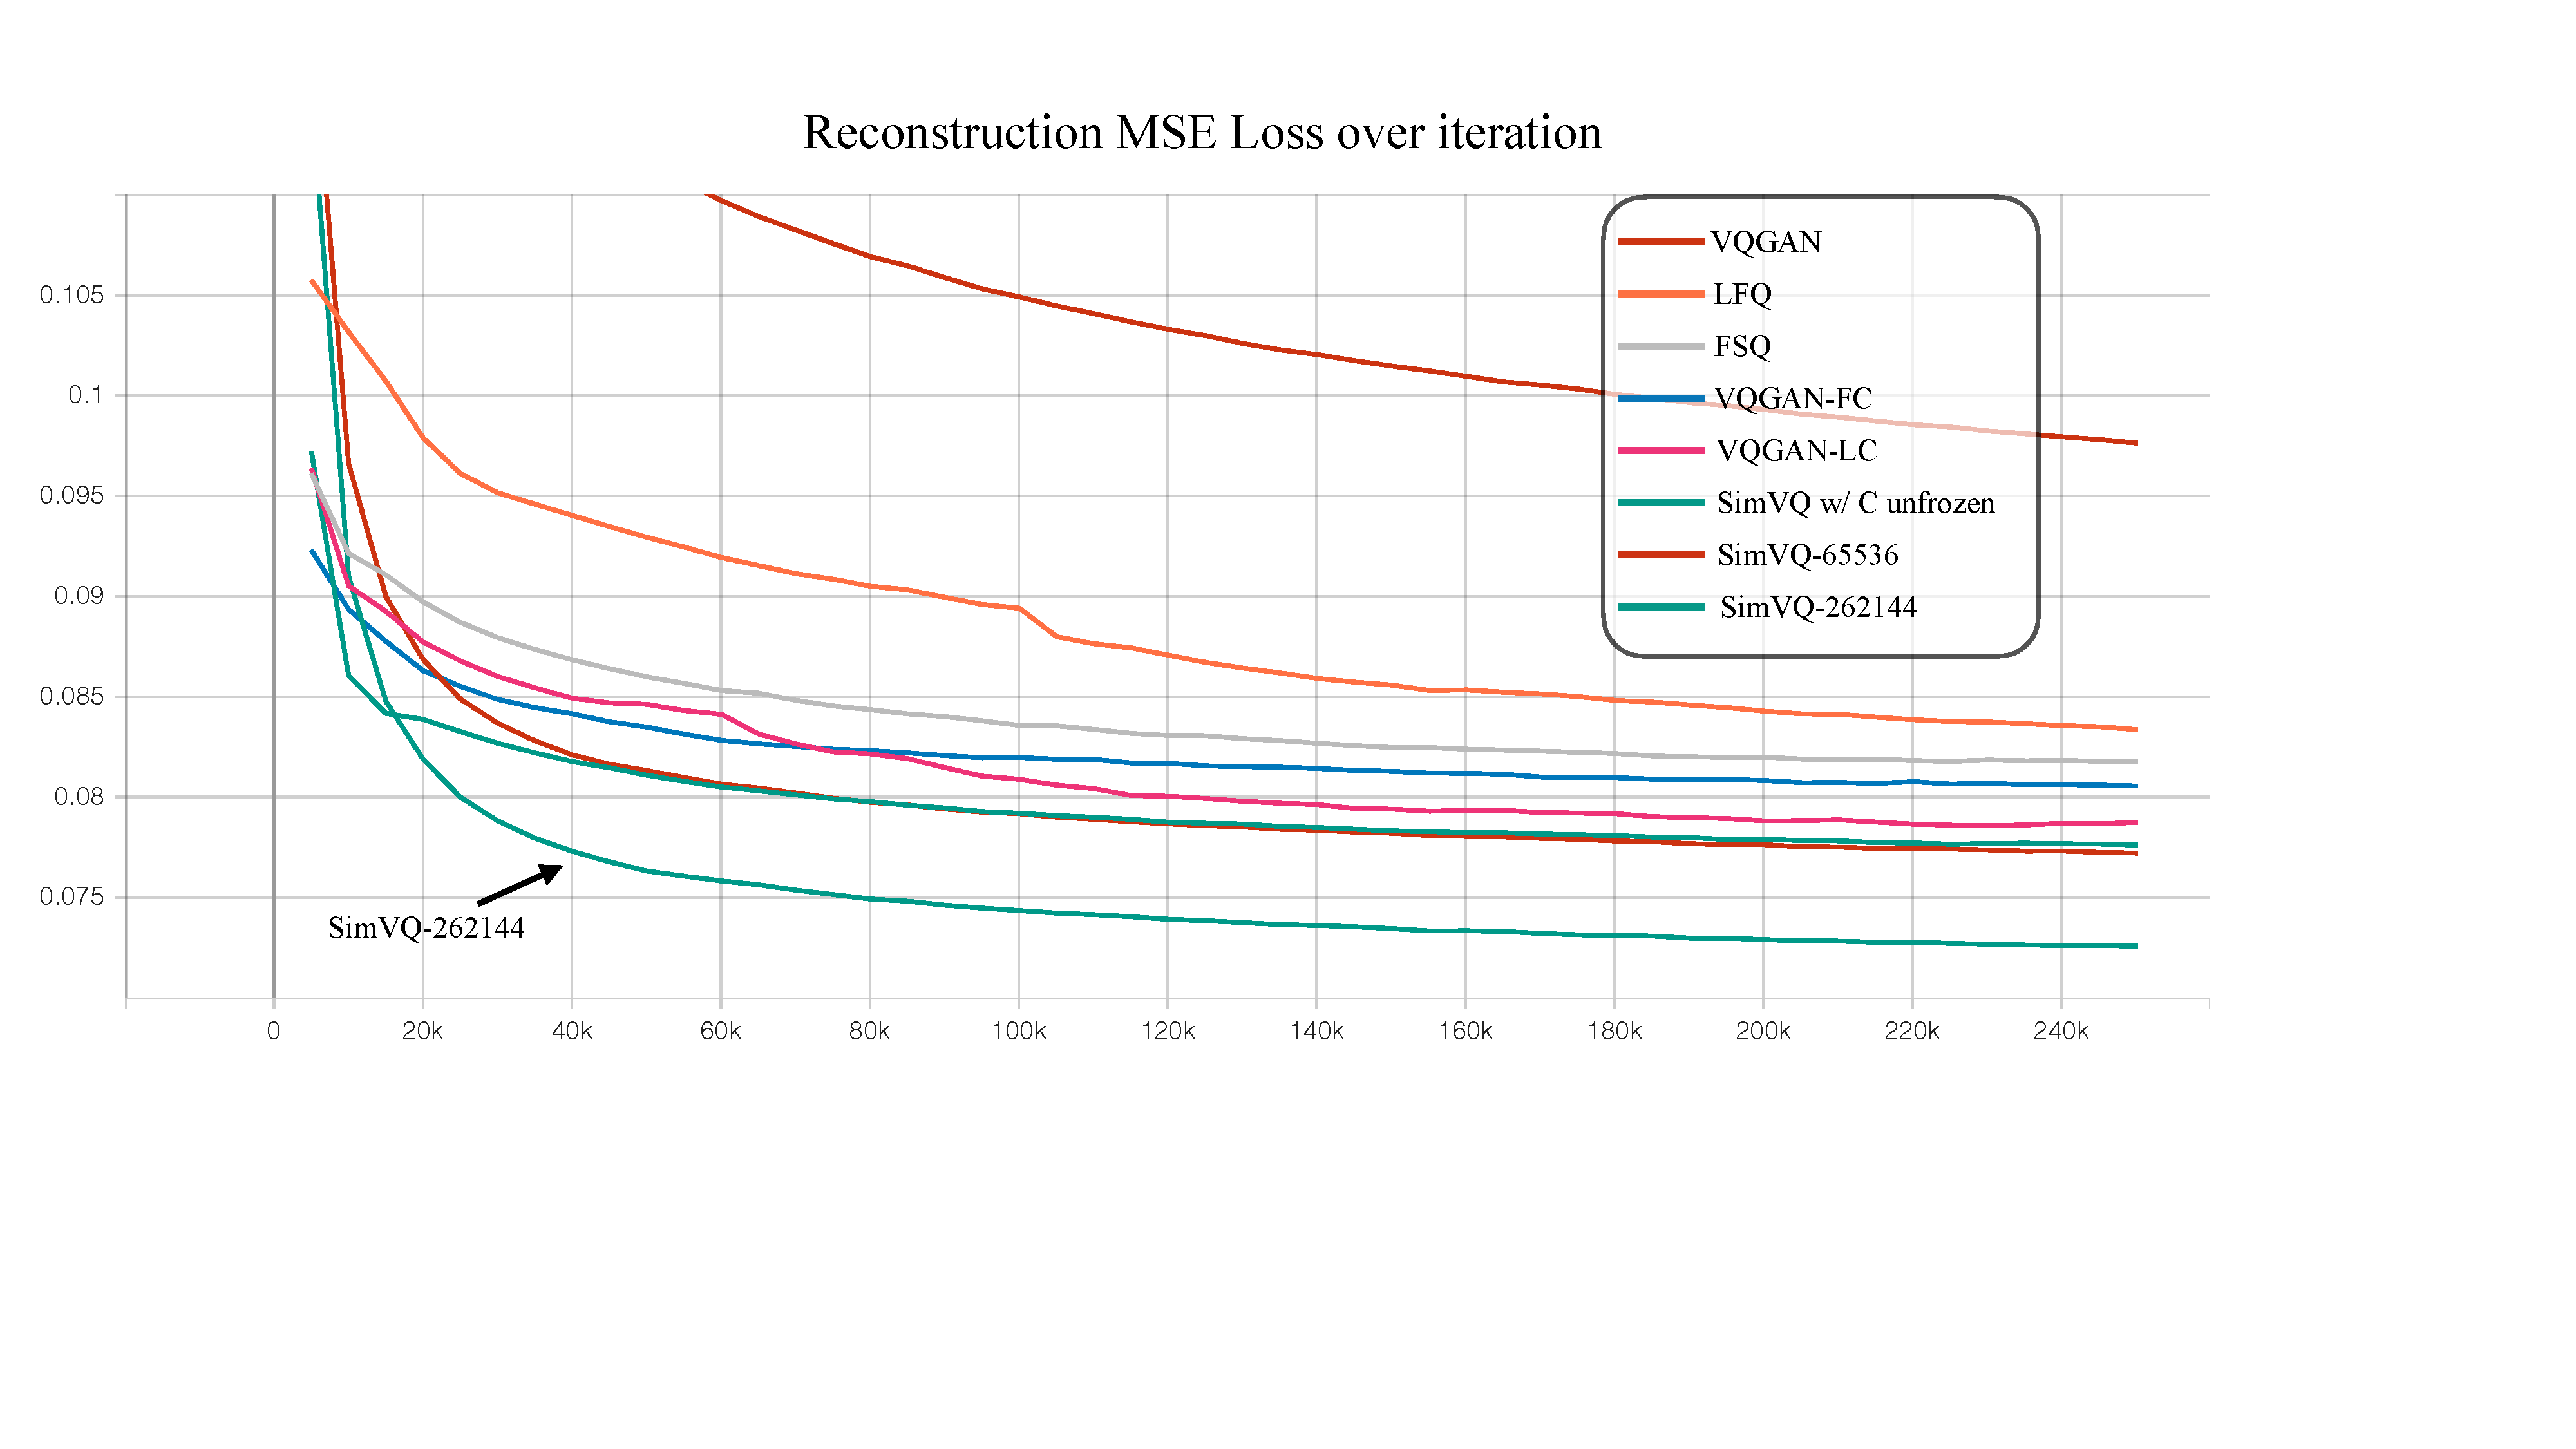
\includegraphics[width=1.0\columnwidth]{material/loss.pdf}
    \caption{The loss curve over epochs of different models on the validation dataset.}
    \label{fig:loss}
\end{figure}


\subsection{Codebook Distribution}
\label{appendix:freq}

\begin{figure}[htb]
    \centering
    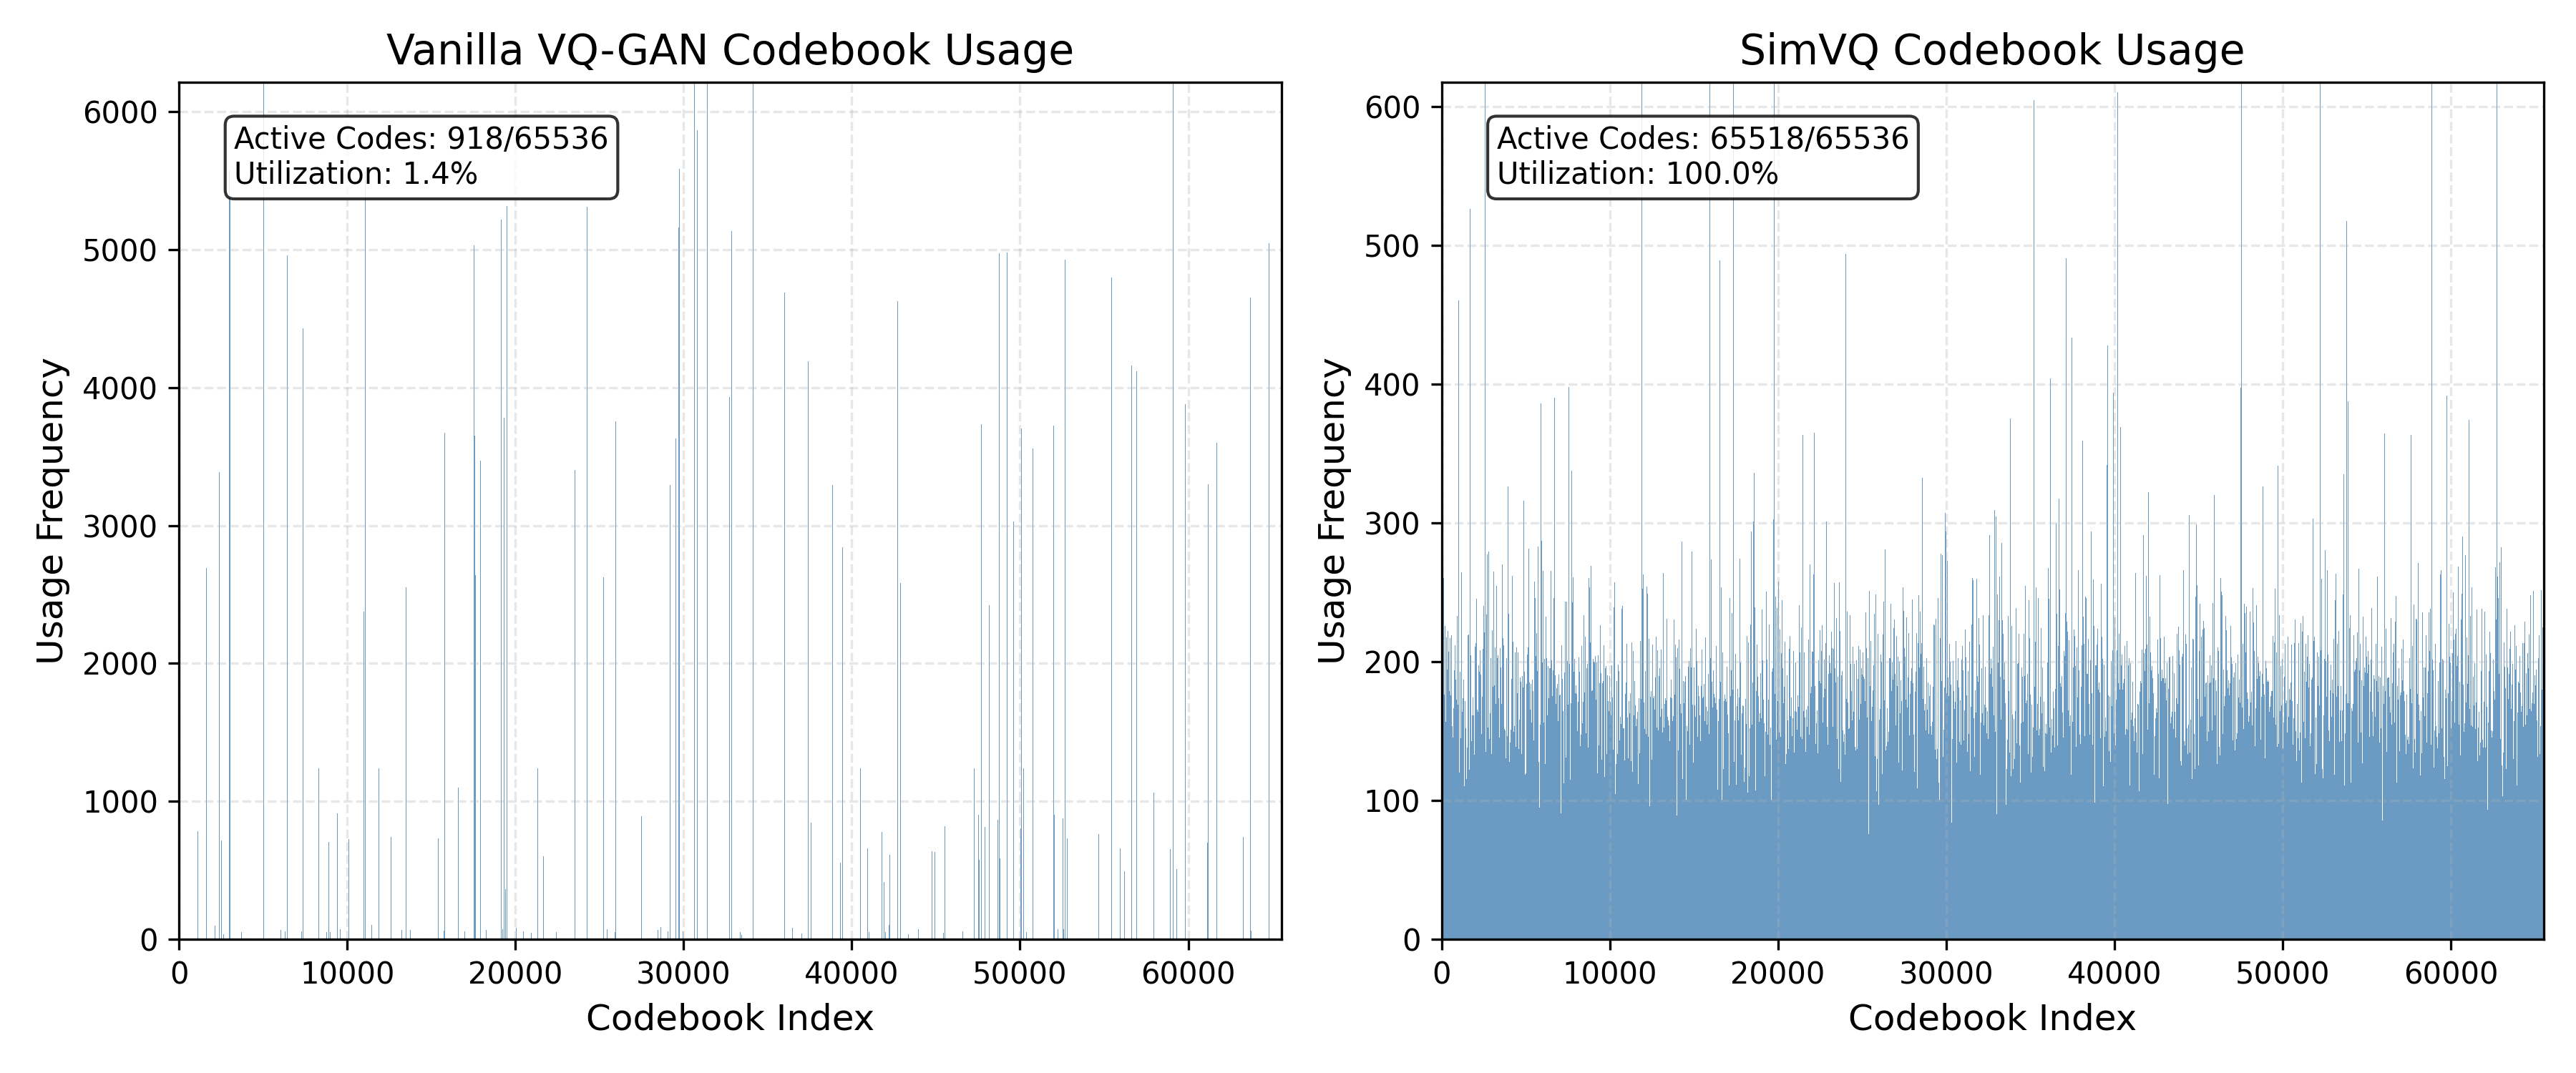
\includegraphics[width=1.0\columnwidth]{material/indices_frequency_comparison.png}
    \caption{The frequency of codebook on ImageNet validation set.}
    \label{fig:freq}
\end{figure}




\subsection{Qualitative Cases}
\label{appendix:cases}

We provide image and audio cases of SimVQ with various codebook sizes below.


\begin{figure*}[h]
    \centering
    {\small
    \makebox[0.16\textwidth]{Origin}%
    \makebox[0.16\textwidth]{vanilla VQ 65,536}%
    \makebox[0.16\textwidth]{SimVQ 1,024}%
    \makebox[0.16\textwidth]{SimVQ 8,192}%
    \makebox[0.16\textwidth]{SimVQ 65,536}%
    \makebox[0.16\textwidth]{SimVQ 262,144}
    }
    \vspace{5pt} 
    
    \begin{minipage}{0.15\textwidth}
        \centering
        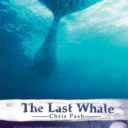
\includegraphics[width=\linewidth]{material/origin/2.png}
    \end{minipage}
    \begin{minipage}{0.15\textwidth}
        \centering
        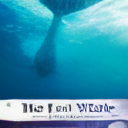
\includegraphics[width=\linewidth]{material/vq/2.png}
    \end{minipage}
    \begin{minipage}{0.15\textwidth}
        \centering
        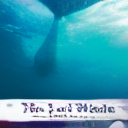
\includegraphics[width=\linewidth]{material/1k/2.png}
    \end{minipage}
    \begin{minipage}{0.15\textwidth}
        \centering
        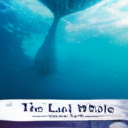
\includegraphics[width=\linewidth]{material/8k/2.png}
    \end{minipage}
    \begin{minipage}{0.15\textwidth}
        \centering
        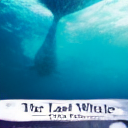
\includegraphics[width=\linewidth]{material/65k/2.png}
    \end{minipage}
    \begin{minipage}{0.15\textwidth}
        \centering
        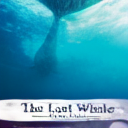
\includegraphics[width=\linewidth]{material/262k/2.png}
    \end{minipage}

    
    % 换行
    \vspace{10pt}
    
    \begin{minipage}{0.15\textwidth}
        \centering
        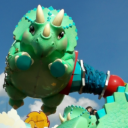
\includegraphics[width=\linewidth]{material/origin/40.png}
    \end{minipage}
    \begin{minipage}{0.15\textwidth}
        \centering
        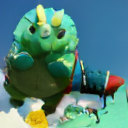
\includegraphics[width=\linewidth]{material/vq/40.png}
    \end{minipage}
    \begin{minipage}{0.15\textwidth}
        \centering
        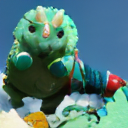
\includegraphics[width=\linewidth]{material/1k/40.png}
    \end{minipage}
    \begin{minipage}{0.15\textwidth}
        \centering
        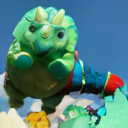
\includegraphics[width=\linewidth]{material/8k/40.png}
    \end{minipage}
    \begin{minipage}{0.15\textwidth}
        \centering
        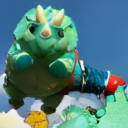
\includegraphics[width=\linewidth]{material/65k/40.png}
    \end{minipage}
    \begin{minipage}{0.15\textwidth}
        \centering
        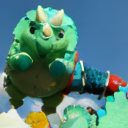
\includegraphics[width=\linewidth]{material/262k/40.png}
    \end{minipage}

    \begin{minipage}{0.15\textwidth}
        \centering
        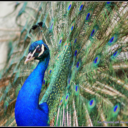
\includegraphics[width=\linewidth]{material/origin/66.png}
    \end{minipage}
    \begin{minipage}{0.15\textwidth}
        \centering
        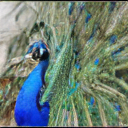
\includegraphics[width=\linewidth]{material/vq/66.png}
    \end{minipage}
    \begin{minipage}{0.15\textwidth}
        \centering
        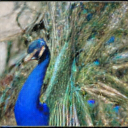
\includegraphics[width=\linewidth]{material/1k/66.png}
    \end{minipage}
    \begin{minipage}{0.15\textwidth}
        \centering
        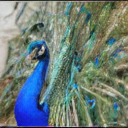
\includegraphics[width=\linewidth]{material/8k/66.png}
    \end{minipage}
    \begin{minipage}{0.15\textwidth}
        \centering
        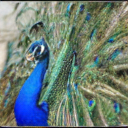
\includegraphics[width=\linewidth]{material/65k/66.png}
    \end{minipage}
    \begin{minipage}{0.15\textwidth}
        \centering
        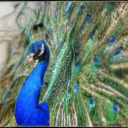
\includegraphics[width=\linewidth]{material/262k/66.png}
    \end{minipage}

    \begin{minipage}{0.15\textwidth}
        \centering
        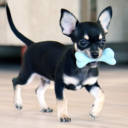
\includegraphics[width=\linewidth]{material/origin/118.png}
    \end{minipage}
    \begin{minipage}{0.15\textwidth}
        \centering
        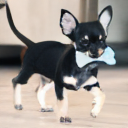
\includegraphics[width=\linewidth]{material/vq/118.png}
    \end{minipage}
    \begin{minipage}{0.15\textwidth}
        \centering
        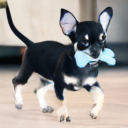
\includegraphics[width=\linewidth]{material/1k/118.png}
    \end{minipage}
    \begin{minipage}{0.15\textwidth}
        \centering
        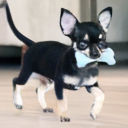
\includegraphics[width=\linewidth]{material/8k/118.png}
    \end{minipage}
    \begin{minipage}{0.15\textwidth}
        \centering
        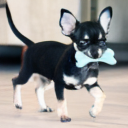
\includegraphics[width=\linewidth]{material/65k/118.png}
    \end{minipage}
    \begin{minipage}{0.15\textwidth}
        \centering
        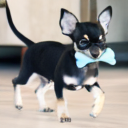
\includegraphics[width=\linewidth]{material/262k/118.png}
    \end{minipage}


    \begin{minipage}{0.15\textwidth}
        \centering
        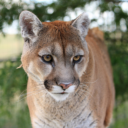
\includegraphics[width=\linewidth]{material/origin/224.png}
    \end{minipage}
    \begin{minipage}{0.15\textwidth}
        \centering
        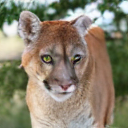
\includegraphics[width=\linewidth]{material/vq/224.png}
    \end{minipage}
    \begin{minipage}{0.15\textwidth}
        \centering
        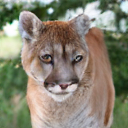
\includegraphics[width=\linewidth]{material/1k/224.png}
    \end{minipage}
    \begin{minipage}{0.15\textwidth}
        \centering
        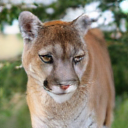
\includegraphics[width=\linewidth]{material/8k/224.png}
    \end{minipage}
    \begin{minipage}{0.15\textwidth}
        \centering
        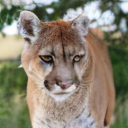
\includegraphics[width=\linewidth]{material/65k/224.png}
    \end{minipage}
    \begin{minipage}{0.15\textwidth}
        \centering
        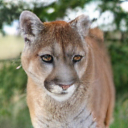
\includegraphics[width=\linewidth]{material/262k/224.png}
    \end{minipage}

    \begin{minipage}{0.15\textwidth}
        \centering
        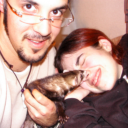
\includegraphics[width=\linewidth]{material/origin/281.png}
    \end{minipage}
    \begin{minipage}{0.15\textwidth}
        \centering
        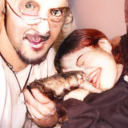
\includegraphics[width=\linewidth]{material/vq/281.png}
    \end{minipage}
    \begin{minipage}{0.15\textwidth}
        \centering
        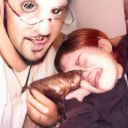
\includegraphics[width=\linewidth]{material/1k/281.png}
    \end{minipage}
    \begin{minipage}{0.15\textwidth}
        \centering
        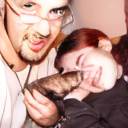
\includegraphics[width=\linewidth]{material/8k/281.png}
    \end{minipage}
    \begin{minipage}{0.15\textwidth}
        \centering
        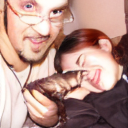
\includegraphics[width=\linewidth]{material/65k/281.png}
    \end{minipage}
    \begin{minipage}{0.15\textwidth}
        \centering
        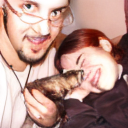
\includegraphics[width=\linewidth]{material/262k/281.png}
    \end{minipage}

    \begin{minipage}{0.15\textwidth}
        \centering
        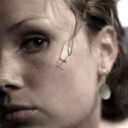
\includegraphics[width=\linewidth]{material/origin/328.png}
    \end{minipage}
    \begin{minipage}{0.15\textwidth}
        \centering
        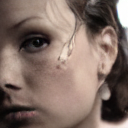
\includegraphics[width=\linewidth]{material/vq/328.png}
    \end{minipage}
    \begin{minipage}{0.15\textwidth}
        \centering
        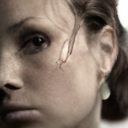
\includegraphics[width=\linewidth]{material/1k/328.png}
    \end{minipage}
    \begin{minipage}{0.15\textwidth}
        \centering
        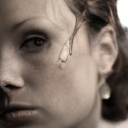
\includegraphics[width=\linewidth]{material/8k/328.png}
    \end{minipage}
    \begin{minipage}{0.15\textwidth}
        \centering
        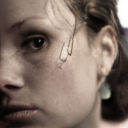
\includegraphics[width=\linewidth]{material/65k/328.png}
    \end{minipage}
    \begin{minipage}{0.15\textwidth}
        \centering
        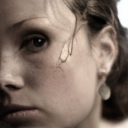
\includegraphics[width=\linewidth]{material/262k/328.png}
    \end{minipage}

    \begin{minipage}{0.15\textwidth}
        \centering
        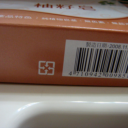
\includegraphics[width=\linewidth]{material/origin/374.png}
    \end{minipage}
    \begin{minipage}{0.15\textwidth}
        \centering
        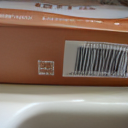
\includegraphics[width=\linewidth]{material/vq/374.png}
    \end{minipage}
    \begin{minipage}{0.15\textwidth}
        \centering
        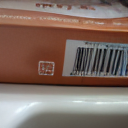
\includegraphics[width=\linewidth]{material/1k/374.png}
    \end{minipage}
    \begin{minipage}{0.15\textwidth}
        \centering
        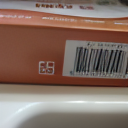
\includegraphics[width=\linewidth]{material/8k/374.png}
    \end{minipage}
    \begin{minipage}{0.15\textwidth}
        \centering
        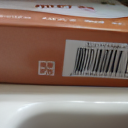
\includegraphics[width=\linewidth]{material/65k/374.png}
    \end{minipage}
    \begin{minipage}{0.15\textwidth}
        \centering
        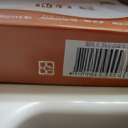
\includegraphics[width=\linewidth]{material/262k/374.png}
    \end{minipage}
    
    \caption{Image reconstruction samples with different codebook sizes.}
\end{figure*}

\begin{figure*}[h]
    \centering
    \includegraphics[width=2.0\columnwidth]{material/spec.png}
    \caption{The spectrogram of audio reconstruction samples with different codebook sizes.}
    \label{fig:spec}
\end{figure*}

\begin{figure*}[h]
    \centering
    \includegraphics[width=2.0\columnwidth]{material/waveform.png}
    \caption{The waveform of audio reconstruction samples with different codebook sizes.}
    \label{fig:waveform}
\end{figure*}
